\chapter{Collections and Persistence}

\section{Introduction to Dynamic Containers}

When designing system-level applications, we frequently encounter scenarios where the volume of data is not known at compile time. Static arrays are insufficient because their size must be defined in advance. We need dynamic containers---data structures that can grow or shrink at runtime. In Rust, these containers allocate memory on the heap and provide safe abstractions for managing it.

This chapter explores Rust's most heavily used dynamic collections: sequences (\texttt{Vec<T>}), associative arrays (\texttt{HashMap<K, V>}), and text containers (\texttt{String}). We will also investigate how to serialize and persist this data to the filesystem using \texttt{PathBuf} and \texttt{File}.


\subsection{Shared Collection API and Complexity}
Regardless of the specific collection type, Rust provides a consistent set of core APIs that are shared across most dynamic containers:
\begin{itemize}
    \item \texttt{new()}: Creates a new, empty collection.
    \item \texttt{with\_capacity(n)}: Preallocates space for \texttt{n} elements, avoiding reallocation costs if the size is known.
    \item \texttt{len()}: Returns the number of elements currently stored.
    \item \texttt{is\_empty()}: Returns \texttt{true} if the collection contains no elements.
    \item \texttt{clear()}: Removes all elements, resulting in an empty collection (often preserving capacity).
    \item \texttt{iter()}: Returns an iterator over references to the elements.
    \item \texttt{into\_iter()}: Disassembles the collection, transferring ownership of the elements to the caller.
    \item \texttt{FromIterator} / \texttt{collect()}: Constructs a collection by consuming an iterator.
\end{itemize}

\begin{table}[h!]
\centering
\begin{tabular}{|l|l|l|l|l|}
\hline
\textbf{Data Structure} & \textbf{Rust} & \textbf{C++} & \textbf{Java} & \textbf{Python} \\
\hline
Dynamic Array & \texttt{Vec<T>} & \texttt{std::vector} & \texttt{ArrayList} & \texttt{list} \\
Double-ended Queue & \texttt{VecDeque<T>} & \texttt{std::deque} & \texttt{ArrayDeque} & \texttt{collections.deque} \\
Linked List & \texttt{LinkedList<T>} & \texttt{std::list} & \texttt{LinkedList} & N/A \\
Hash Map & \texttt{HashMap<K, V>} & \texttt{std::unordered\_map} & \texttt{HashMap} & \texttt{dict} \\
Ordered Map & \texttt{BTreeMap<K, V>} & \texttt{std::map} & \texttt{TreeMap} & N/A \\
Hash Set & \texttt{HashSet<T>} & \texttt{std::unordered\_set} & \texttt{HashSet} & \texttt{set} \\
Ordered Set & \texttt{BTreeSet<T>} & \texttt{std::set} & \texttt{TreeSet} & N/A \\
Priority Queue & \texttt{BinaryHeap<T>} & \texttt{std::priority\_queue} & \texttt{PriorityQueue} & \texttt{heapq} \\
\hline
\end{tabular}
\caption{Equivalent Collections Across Programming Languages}
\label{tab:collections_comparison}
\end{table}

\begin{insightbox}[Understanding Computational Complexity]
The professor emphasizes understanding the Big-O complexity for various collection operations to make informed architectural decisions:
\begin{itemize}
    \item \textbf{$O(1)$ (Constant time):} The operation takes the same amount of time regardless of the container size.
    \item \textbf{Amortized $O(1)$:} Most operations are $O(1)$, but occasionally a more expensive operation occurs (e.g., reallocating a \texttt{Vec}'s buffer). Over many operations, the average cost remains $O(1)$.
    \item \textbf{$O(\log N)$ (Logarithmic time):} The execution time grows logarithmically. It grows very slowly even for large datasets (e.g., operations on a \texttt{BTreeMap}).
    \item \textbf{$O(N)$ (Linear time):} The time scales directly with the number of elements (e.g., inserting into the middle of a \texttt{Vec}).
    \item \textbf{$O(N \log N)$ (Linearithmic time):} Typical complexity for efficient sorting algorithms like Quicksort or Mergesort.
\end{itemize}
\end{insightbox}


\section{Sequences: Vectors (\texttt{Vec<T>})}

\subsection{The Problem of Contiguous Dynamic Data}
Imagine you are reading lines from a log file. You do not know how many lines exist until you reach the end of the file. You need a data structure that keeps elements in a sequence, allows rapid sequential access, and can expand its capacity on demand. 

\subsection{Mechanism and Memory Layout}
The standard solution in Rust is the \texttt{Vec<T>} (vector). A vector ensures that all its elements of type \texttt{T} are contiguous in memory.

Under the hood, a \texttt{Vec<T>} consists of three fields (one pointer and two integers), as illustrated below:

\begin{figure}[H]
    \centering
    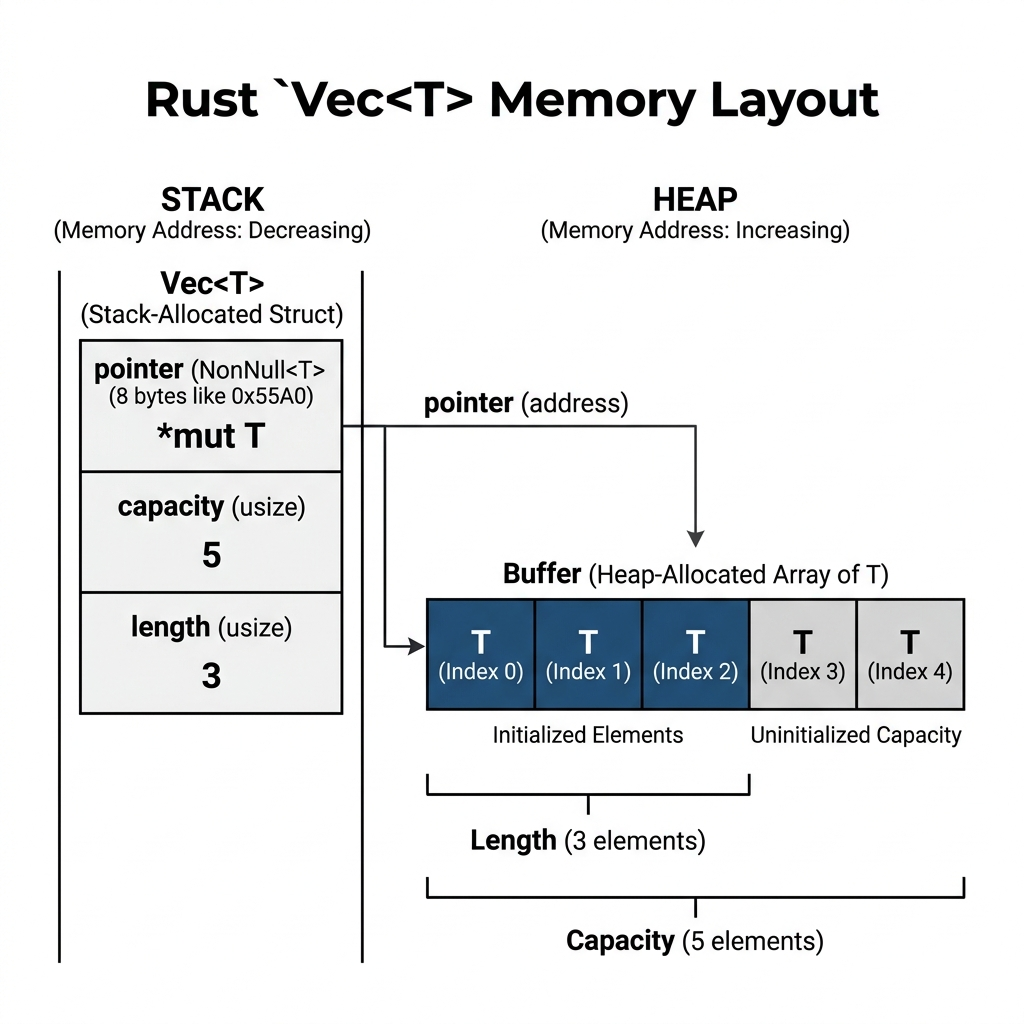
\includegraphics[width=0.7\textwidth]{images/vec_three_components.png}
    \caption{The three core components of a \texttt{Vec<T>}: pointer, capacity, and length.}
    \label{fig:vec_components}
\end{figure}

\begin{itemize}
    \item A \textbf{pointer} to the heap-allocated buffer containing the data.
    \item The \textbf{capacity}: how much space is currently allocated.
    \item The \textbf{length}: how many elements are currently instantiated.
\end{itemize}

When you push an element onto a vector, it occupies the next free slot in the pre-allocated buffer. If the length reaches the capacity, the vector must \textit{reallocate}: it requests a larger block of memory (usually double the size), copies the existing elements over, and deallocates the old buffer.


\begin{insightbox}[Sorting and Slicing Advantages]
The contiguous memory layout of a \texttt{Vec} provides two major advantages:
\begin{itemize}
    \item \textbf{Sorting:} Sorting algorithms perform exceptionally well on contiguous memory. If you store elements non-contiguously, sorting becomes significantly more expensive.
    \item \textbf{Slicing:} Creating a slice from a vector is an $O(1)$ operation because it simply requires extracting a pointer to the start and a length.
\end{itemize}
\end{insightbox}

\subsection{Concrete Example: Building a Vector}
Let us examine the basic usage of a vector:

\begin{lstlisting}[language=Rust]
let mut numbers: Vec<i32> = Vec::new(); // Length: 0, Capacity: 0

// Pushing elements allocates memory on the heap
numbers.push(10);
numbers.push(20);
numbers.push(30);

println!("First element: {}", numbers[0]);

// Popping removes the last element (30)
if let Some(last) = numbers.pop() {
    println!("Removed: {}", last);
}
\end{lstlisting}

\paragraph{Memory Model Analysis:}
The variable \texttt{numbers} itself is allocated on the stack, consisting of three machine words: a pointer to the heap, the capacity, and the length. Initially, the heap pointer might be null or a dangling placeholder because \texttt{Vec::new()} does not allocate. When \texttt{push(10)} is called, Rust requests heap memory to store the elements. The \texttt{numbers} stack structure is mutated to update its capacity, length, and the pointer to the newly allocated heap block. As elements are pushed, ownership of the values moves into the \texttt{Vec}'s heap allocation. When \texttt{numbers} goes out of scope, its \texttt{Drop} implementation will be called, deallocating the heap buffer before popping the stack frame.

\begin{notebox}[Optimizing Allocations]
Reallocation is an expensive $O(N)$ operation. If you know approximately how many elements you will store, you should use \texttt{Vec::with\_capacity(n)}. This allocates the necessary memory upfront, significantly amortizing the cost of insertion to $O(1)$.
\end{notebox}

\subsection{Trade-offs}
Vectors are highly efficient for inserting or removing at the \emph{end} (\texttt{push}/\texttt{pop}) and provide excellent CPU cache locality due to their contiguous layout. However, inserting or removing elements at the \emph{front} or in the \emph{middle} forces all subsequent elements to shift, resulting in an $O(N)$ cost. 
In addition to \texttt{push} and \texttt{pop}, vectors provide \texttt{insert(index, element)} and \texttt{remove(index)}. However, using these methods requires shifting all subsequent elements, introducing an $O(N)$ cost per operation.


\textbf{When and why to use it:} Use \texttt{Vec<T>} by default for sequences when you need fast random access by index, cache-friendly iteration, and mostly append-only insertions.

\subsection{Heterogeneous Sequences via Enums}
While a \texttt{Vec<T>} strictly requires all elements to be of the same type \texttt{T}, you can elegantly store heterogeneous data by defining an \texttt{enum}. By wrapping different data types in enum variants, the vector remains technically homogeneous, but logically heterogeneous:

\begin{lstlisting}[language=Rust]
enum SpreadsheetCell {
    Int(i32),
    Float(f64),
    Text(String),
}

let row = vec![
    SpreadsheetCell::Int(3),
    SpreadsheetCell::Text(String::from("blue")),
    SpreadsheetCell::Float(10.12),
];
\end{lstlisting}

\section{Sequences: Double-Ended Queues (\texttt{VecDeque<T>})}

When operations at both ends of a sequence are frequent (such as in a FIFO queue or a sliding window), \texttt{VecDeque} is the ideal choice. 

\subsection{Mechanism and Memory Layout}
Unlike \texttt{Vec}, which only efficiently grows at the tail, a \texttt{VecDeque} is implemented as a \textbf{ring buffer}. It allocates a contiguous block of memory on the heap (just like a \texttt{Vec}), but it maintains two distinct indices: a \texttt{head} and a \texttt{tail}.

\begin{figure}[H]
    \centering
    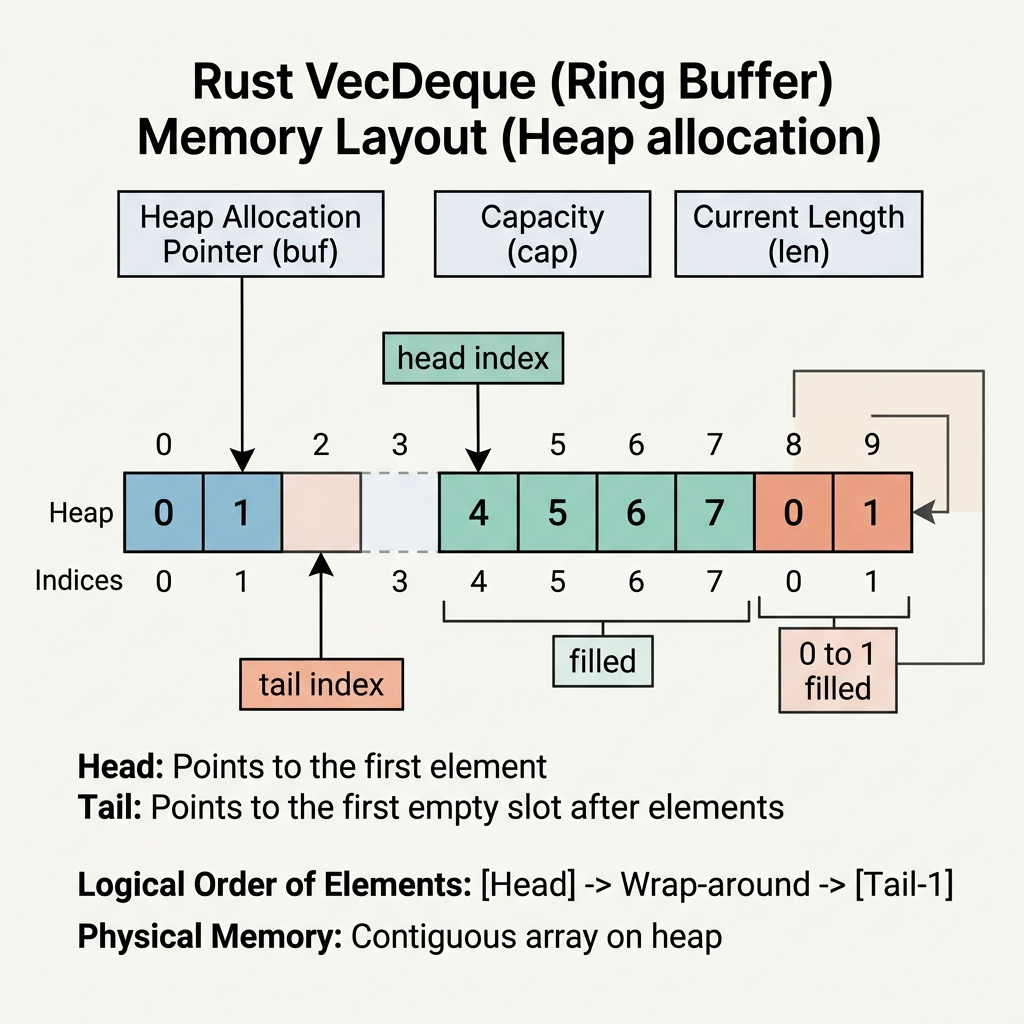
\includegraphics[width=0.7\textwidth]{images/vecdeque_ring_buffer.png}
    \caption{The ring buffer memory layout of a \texttt{VecDeque}. Elements can wrap around the end of the allocated heap space back to the beginning.}
    \label{fig:vecdeque_memory}
\end{figure}

Because it tracks both ends, it achieves \textbf{$O(1)$ constant time insertions and removals at both ends}. If you push an element to the front, the \texttt{head} index simply decrements. If it hits the start of the allocated buffer, it mathematically ``wraps around'' to the very end of the buffer space. No existing elements need to be shifted in memory. Shifting and reallocation only occur if the ring buffer becomes completely full.

Since the elements might wrap around the buffer, they are not always strictly contiguous in physical memory order from the perspective of a slice. You can, however, force them to be physically contiguous using the \texttt{make\_contiguous()} method.

\textbf{When and why to use it:} Use \texttt{VecDeque} when implementing a FIFO queue or maintaining a sliding window of recent elements where frequent insertions and removals occur at both ends.

\section{Sequences: Linked Lists (\texttt{LinkedList<T>})}

Rust also provides a doubly linked list, \texttt{LinkedList<T>}. 

\subsection{Mechanism and Memory Layout}
Unlike \texttt{Vec} and \texttt{VecDeque}, a linked list does not use a single contiguous block of heap memory. Instead, every single element inserted into the list is wrapped in a \texttt{Node} struct, which is allocated entirely on its own on the heap.

\begin{figure}[H]
    \centering
    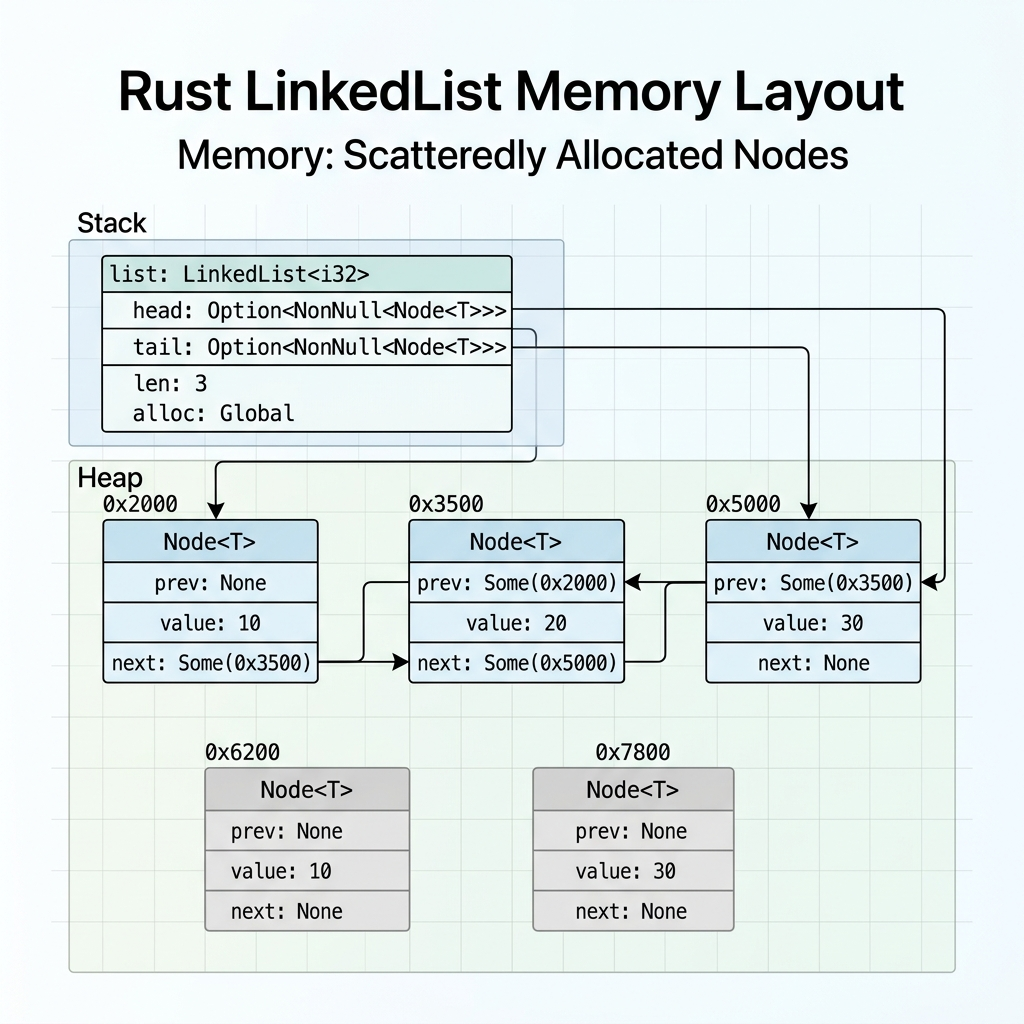
\includegraphics[width=0.7\textwidth]{images/linkedlist_memory_layout.png}
    \caption{The doubly linked list memory layout. Nodes are scattered across the heap, connected by \texttt{prev} and \texttt{next} pointers.}
    \label{fig:linkedlist_memory}
\end{figure}

Each node contains three components: a pointer to the previous node, the actual value, and a pointer to the next node. 
Because nodes are physically independent, inserting an element at the front or back guarantees a strictly \textbf{$O(1)$ constant time cost}. The system simply allocates a new node on the heap and updates the \texttt{next}/\texttt{prev} pointers of the existing head or tail to include the new node. Absolutely no shifting of existing elements is required.

\subsection{Trade-offs}
However, due to nodes being scattered randomly across the heap, \texttt{LinkedList} suffers from a high probability of \textbf{cache misses}. When the processor attempts to iterate through the list, fetching the next node likely requires querying the much slower main RAM rather than the ultra-fast CPU cache. Furthermore, accessing an arbitrary element by index requires traversing the list node-by-node, resulting in an $O(N)$ access time.

\textbf{When and why to use it:} Use \texttt{LinkedList<T>} almost exclusively when you need constant time $O(1)$ concatenation of two lists or splitting a list at a known node without allocating, especially in real-time systems where reallocation latency is unacceptable. It is rarely used for general-purpose programming.

\section{Text Collections: \texttt{String} vs \texttt{\&str}}

Strings are among the most misunderstood collections in Rust. To write robust systems code, you must build a solid mental model distinguishing between \texttt{String} and \texttt{\&str}.

\subsection{Building Intuition}
Think of a \texttt{String} exactly like a \texttt{Vec<u8>}. In fact, a \texttt{String} is simply a wrapper over a vector of bytes that guarantees the bytes form a valid UTF-8 sequence. Since it owns its data on the heap, you can grow it, mutate it, and append to it.

Conversely, an \texttt{\&str} (string slice) is a borrowed view into some UTF-8 data. It consists of a pointer to the start of the text and a length. It does not own the data, and it cannot grow or shrink.

\begin{examprioritybox}
\textbf{Common Pitfall:} Unnecessarily taking ownership by using \texttt{String} as a function parameter when a read-only \texttt{\&str} view would suffice, leading to wasteful heap allocations.

\textbf{Expected Mastery Level:} Very High. A fundamental exam topic is choosing the correct string type:
\begin{itemize}
    \item Use \texttt{String} when you need to \textbf{own} the text data or modify it (e.g., concatenating input, reading from a file).
    \item Use \texttt{\&str} when you only need to \textbf{read} or view the text (e.g., passing a string as an argument to a function). This avoids unnecessary heap allocations.
\end{itemize}
\end{examprioritybox}

\subsection{Concrete Example: Conversions}

\begin{lstlisting}[language=Rust]
// s1 is an &str pointing to read-only memory (the binary itself)
let s1: &str = "Hello, world!";

// We create an owned String allocated on the heap
let mut s2: String = String::from(s1);

// We can mutate the String
s2.push_str(" I am learning Rust.");

// We can extract a view (&str) from the String
let view: &str = &s2[0..5]; // "Hello"
\end{lstlisting}

\paragraph{Memory Model Analysis:}
\texttt{s1} is a fat pointer (\texttt{ptr}, \texttt{len}) residing on the stack, pointing to the \texttt{.rodata} segment of the compiled binary; it represents an immutable borrow with a \texttt{'static} lifetime. When creating \texttt{s2}, Rust allocates a new buffer on the heap and copies the bytes from \texttt{s1}. \texttt{s2} is an owned \texttt{String} (a stack structure with \texttt{ptr}, \texttt{len}, \texttt{capacity}). Calling \texttt{push\_str} may trigger a heap reallocation if the new text exceeds the current capacity. Finally, \texttt{view} is another \texttt{\&str} fat pointer on the stack, but this time its pointer points into the heap buffer owned by \texttt{s2}, and its lifetime is tied to the scope of \texttt{s2}. If \texttt{s2} is dropped or mutated further, \texttt{view} becomes invalid, which the borrow checker enforces at compile time.

\section{Maps, Sets, and Priority Queues}

\subsection{The Problem of Fast Lookup}
While vectors are excellent for sequential data, they are extremely inefficient if we need to search for an element by an arbitrary identifier (like a username or a product ID). A linear search takes $O(N)$ time. We need a structure that provides $O(1)$ expected lookup times.

\subsection{Mechanism: Hashing and Buckets}
The \texttt{HashMap<K, V>} associates keys of type \texttt{K} with values of type \texttt{V}. When a key is inserted, it passes through a \textit{hash function}, producing a semi-random integer (the hash). This integer is used to index into a series of "buckets".

\begin{figure}[h!]
    \centering
    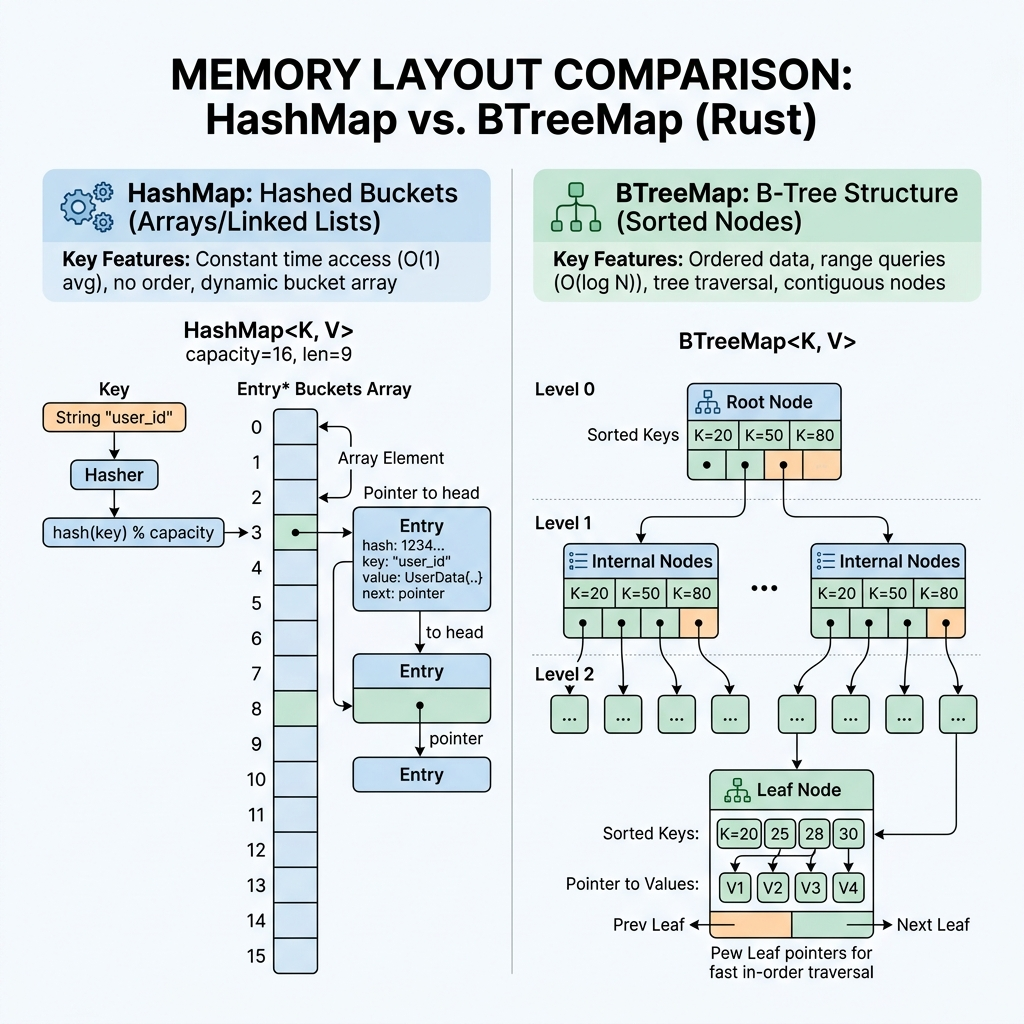
\includegraphics[width=0.7\textwidth]{images/hashmap_layout.png}
    \caption{Memory Layout and Hashing Mechanism in a HashMap}
    \label{fig:hashmap_layout}
\end{figure}

As shown in Figure~\ref{fig:hashmap_layout}, if multiple keys map to the same bucket (a collision), they are stored linearly inside that bucket. For the map to function correctly, keys must implement two traits:
\begin{itemize}
    \item \texttt{Hash}: to convert the key into a number.
    \item \texttt{Eq}: to precisely check for equality in case of collisions.
\end{itemize}

\begin{examprioritybox}
\textbf{Common Pitfall:} Assuming \texttt{HashMap} iteration order is predictable, or using types with internal mutability (e.g., \texttt{RefCell}) as keys, breaking invariants.

\textbf{Expected Mastery Level:} Very High. You must know when to choose \texttt{HashMap} ($O(1)$ expected, unordered) versus \texttt{BTreeMap} ($O(\log N)$, ordered). You also must know that \texttt{HashMap} requires \texttt{Hash} and \texttt{Eq}, while \texttt{BTreeMap} requires \texttt{Ord}, and that these implementations must be logically consistent.

Iterating over a \texttt{HashMap} yields keys and values in an unpredictable order. If you need ordered iteration, use a \texttt{BTreeMap} instead, which stores elements in a balanced search tree at the cost of $O(\log N)$ access time. Furthermore, keys in any map must remain immutable while they are stored.
\end{examprioritybox}


\begin{insightbox}[Consistent Traits and Internal Mutability]
Just like \texttt{hashCode} and \texttt{equals} in Java, the \texttt{Hash} and \texttt{Eq} traits in Rust \textbf{must be logically consistent}. If two objects are equal (\texttt{Eq}), they must produce the same hash. Furthermore, a good hash function should evenly distribute values to avoid turning bucket lookups into $O(N)$ linear searches.

Crucially, \textbf{keys must remain stable}. You cannot use objects with internal mutability (like \texttt{RefCell}) as keys in a map, because mutating the key after insertion would corrupt the map's internal layout.
\end{insightbox}

\subsection{Map Initialization and Filtering}
Unlike \texttt{Vec}, which has the handy \texttt{vec![]} macro, there is no standard macro for initializing maps (because the choice between \texttt{HashMap} and \texttt{BTreeMap} is often balanced, so the language designers preferred explicit instantiation). Instead, you initialize them using the \texttt{From} trait with an array of tuples:

\begin{lstlisting}[language=Rust]
use std::collections::HashMap;

let mut scores = HashMap::from([
    (String::from("Alice"), 80),
    (String::from("Bob"), 90),
    (String::from("Carol"), 70),
]);
\end{lstlisting}

Rust maps also provide excellent methods for filtering in-place:
\begin{itemize}
    \item \textbf{\texttt{retain(|key, \&mut value| ... )}}: Keeps only elements for which the closure returns \texttt{true}.
    \item \textbf{\texttt{remove(key)}}: Removes a specific key. 
\end{itemize}

When iterating, you can use \texttt{into\_iter()} to completely disassemble the map, taking ownership of the key-value tuples.

\subsection{Concrete Example: The Entry API}
Rust's \texttt{HashMap} exposes an incredibly elegant \texttt{Entry} API for updating values conditionally.

\begin{lstlisting}[language=Rust]
use std::collections::HashMap;

let mut scores = HashMap::new();
scores.insert(String::from("Alice"), 50);

// Using the Entry API: Insert "Bob" if he does not exist.
scores.entry(String::from("Bob")).or_insert(30);

// Update Alice's score safely
scores.entry(String::from("Alice")).and_modify(|score| *score += 10);
\end{lstlisting}

\paragraph{Memory Model Analysis:}
The \texttt{HashMap} \texttt{scores} is allocated on the stack, maintaining state about its heap-allocated hash table. When we call \texttt{String::from("Alice")}, a heap allocation occurs for the string data. The map takes ownership of this string, transferring the ownership from the caller to the heap-allocated bucket of the map. The \texttt{entry} method borrows \texttt{scores} mutably, and if the key is not found, \texttt{or\_insert} consumes the \texttt{String} (moving its ownership to the map). The closure passed to \texttt{and\_modify} takes a mutable borrow \texttt{\&mut V} of the value residing in the map's heap, allowing us to safely mutate it in place without extracting it.

The \texttt{Entry} API avoids checking the map twice (once to see if the key exists, and once to insert/update), which improves both performance and readability.

\subsection{Sets: \texttt{HashSet} and \texttt{BTreeSet}}
When you only care about the presence of an element rather than a key-value association, you can use a set. A \texttt{HashSet<T>} is conceptually a \texttt{HashMap<T, ()>} and is perfect for deduplication or mathematical set operations (union, intersection, difference) in expected $O(1)$ time.

\textbf{When and why to use it:} Use \texttt{HashSet} for fast duplicate removal, fast membership checks, and set math operations where iteration order does not matter.

Its ordered counterpart, \texttt{BTreeSet<T>}, requires elements to implement \texttt{Ord} and is ideal when you need to extract ranges of values or iterate in a guaranteed order.

\textbf{When and why to use it:} Use \texttt{BTreeSet} when you need to iterate over unique elements in a deterministic order or need to efficiently query a range of elements.

\subsection{Priority Queues: \texttt{BinaryHeap}}
Sometimes you do not need to keep all elements perfectly sorted, but you frequently need to extract the "most important" or "heaviest" element. A \texttt{BinaryHeap<T>} provides a priority queue where the maximum element is always kept at the top. Peeking the top element is $O(1)$, while pushing or popping costs $O(\log N)$. It relies on the \texttt{Ord} trait to determine priority. 
To implement a Min-Heap (where the smallest/lightest element is extracted first, e.g., in Dijkstra's shortest path algorithm), you must invert the ordering logic. Rather than writing a custom \texttt{Ord} implementation, it is much easier to wrap your elements in \texttt{std::cmp::Reverse<T>}.


\textbf{When and why to use it:} Use \texttt{BinaryHeap} to implement task schedulers, find the top-K elements without sorting the entire dataset, or implement algorithms like Dijkstra's shortest path.

\section{Persistence: \texttt{Path}, \texttt{PathBuf}, and \texttt{File}}

Once we have accumulated data in memory via collections, we usually need to save it to disk. Rust handles filesystem abstractions via the \texttt{std::fs} and \texttt{std::path} modules.

\subsection{Paths: \texttt{PathBuf} vs \texttt{Path}}
Similar to the dichotomy between \texttt{String} and \texttt{\&str}, Rust separates file paths into owned and borrowed types. 
Why not just use a \texttt{String} for a path? Because path separators (\texttt{/} on Unix, \texttt{\char`\\} on Windows) and encoding rules differ strictly across operating systems. A \texttt{Path} guarantees correct, cross-platform path semantics.

\begin{itemize}
    \item \textbf{\texttt{PathBuf}}: The owned, heap-allocated, mutable equivalent of \texttt{String}. You use this when you need to construct or modify a path dynamically.
    \item \textbf{\texttt{\&Path}}: The borrowed equivalent of \texttt{\&str}. Used to pass a read-only path to functions.
\end{itemize}

\begin{lstlisting}[language=Rust]
use std::path::PathBuf;

// Building a path cross-platform
let mut config_path = PathBuf::from("/etc");
config_path.push("app");          // Joins correctly: /etc/app
config_path.push("config.json");  // /etc/app/config.json

// Displaying the path safely
println!("Config file is at: {}", config_path.display());
\end{lstlisting}


\begin{insightbox}[Path Tokenization]
Paths have intrinsic tokenization. A \texttt{Path} is aware of OS-specific separators (\texttt{/} on Unix, \texttt{\char`\\} on Windows) and treats them as boundaries between directory components. This makes navigating directories (e.g., getting the parent or filename) robust.
\end{insightbox}

\subsection{File System Utility Functions}
The \texttt{std::fs} module provides various functions for interacting with the file system itself (not just the contents of files):
\begin{itemize}
    \item \textbf{\texttt{read\_dir}}: Returns an iterator over the entries within a directory.
    \item \textbf{\texttt{create\_dir}} / \textbf{\texttt{remove\_dir}}: Creates or removes an empty directory.
    \item \textbf{\texttt{copy}}: Duplicates a file.
    \item \textbf{\texttt{rename}}: Renames or moves a file. Note that \texttt{rename} behavior depends heavily on the OS, especially when moving files across different mounted disks.
    \item \textbf{\texttt{remove\_file}}: Deletes a file.
\end{itemize}

\subsection{File System Operations and I/O Traits}
The \texttt{std::fs::File} struct represents an open file on the operating system. When a \texttt{File} goes out of scope, Rust automatically closes the file descriptor (leveraging RAII), preventing resource leaks. 


Rust models Input/Output operations through four core traits in the \texttt{std::io} module:

\begin{itemize}
    \item \textbf{\texttt{Read}}: Implemented by \texttt{File}, \texttt{TcpStream}, and \texttt{Stdin}. It provides methods to consume byte streams:
    \begin{itemize}
        \item \texttt{read()}: Reads a chunk of bytes.
        \item \texttt{read\_to\_end()}: Reads all bytes into a \texttt{Vec<u8>}.
        \item \texttt{read\_to\_string()}: Reads the entire file into a UTF-8 \texttt{String}.
        \item \texttt{read\_exact()}: Guarantees filling a pre-sized buffer exactly, useful for reading fixed-length binary records.
        \item \texttt{bytes()}, \texttt{chain()}, \texttt{take()}: Utility adapters for iteration and composing streams.
    \end{itemize}

    \item \textbf{\texttt{Write}}: Implemented by \texttt{File}, \texttt{TcpStream}, \texttt{Stdout}, and \texttt{Stderr}. 
    \begin{itemize}
        \item \texttt{write()}: Attempts to write a buffer. Might be partial.
        \item \texttt{write\_all()}: Writes the entire buffer.
        \item \texttt{flush()}: Forces the operating system to physically push its internal buffers to the persistent disk. 
    \end{itemize}

    \item \textbf{\texttt{BufRead}}: A sub-trait of \texttt{Read} that manages an internal buffer to minimize expensive user-to-kernel mode context switches. It is implemented by \texttt{BufReader}, \texttt{Cursor}, and \texttt{StdinLock}.
    \begin{itemize}
        \item \texttt{fill\_buf()}: Fills the internal buffer.
        \item \texttt{consume(n)}: Marks \texttt{n} bytes as read from the buffer.
        \item \texttt{read\_line()} and \texttt{lines()}: Reads up to the next newline character.
    \end{itemize}

    \item \textbf{\texttt{Seek}}: Allows manipulating the file cursor. Implemented by \texttt{File} and \texttt{Cursor}, but notably \emph{not} by \texttt{TcpStream} (since network streams are not replayable).
    \begin{itemize}
        \item \texttt{seek(pos)}: Moves the cursor relative to the start, end, or current position.
        \item \texttt{rewind()}: Resets the cursor to the beginning (equivalent to \texttt{seek(0)}).
        \item \texttt{stream\_position()}: Returns the current cursor offset.
    \end{itemize}
\end{itemize}


\begin{lstlisting}[language=Rust]
use std::fs::File;
use std::io::{Write, Read, BufReader, BufRead};
use std::path::Path;

// Writing to a file
let path = Path::new("data.txt");
// File::create truncates the file if it exists, or creates it
let mut file = File::create(&path).expect("Failed to create file");
file.write_all(b"Hello from Rust!\nSecond line").expect("Failed to write");

// Reading from a file with a buffer
let input = File::open(&path).expect("Failed to open file");
let buffered = BufReader::new(input);

for line in buffered.lines() {
    println!("{}", line.expect("Failed to read line"));
}
\end{lstlisting}

\paragraph{Memory Model Analysis:}
The \texttt{path} variable is a reference \texttt{\&Path} (a fat pointer) on the stack, pointing to the string literal's static memory. When calling \texttt{File::create}, the OS allocates a file descriptor and returns it; the stack variable \texttt{file} takes ownership of this OS resource. The string literal \texttt{b"..."} is a slice \texttt{\&[u8]} pointing to the read-only memory. In the reading phase, \texttt{BufReader} allocates a heap buffer to fetch chunks of data at once, minimizing expensive syscalls. The \texttt{lines()} iterator creates a new \texttt{String} (heap allocation) for each line parsed, transferring ownership of each line to the loop variable \texttt{line} inside the \texttt{Result}. Finally, RAII automatically closes both \texttt{file} and \texttt{input} when they go out of scope.

\begin{notebox}[Advanced Open Options]
For more precise control (such as appending to a file instead of truncating), you can use \texttt{std::fs::OpenOptions}, which allows explicit combinations of \texttt{read}, \texttt{write}, \texttt{append}, and \texttt{create} flags.
\end{notebox}


\subsection{Error Handling in I/O}
Virtually all I/O operations return a \texttt{std::io::Result<T>}. In case of an error, it returns a \texttt{std::io::Error}, which contains an \texttt{ErrorKind} enum. Checking the \texttt{ErrorKind} allows your application to intelligently recover. 
Common error kinds include:
\begin{itemize}
    \item \texttt{Interrupted}: The OS interrupted the operation; you can safely retry it.
    \item \texttt{PermissionDenied}: The user lacks OS rights.
    \item \texttt{UnexpectedEof}: Reached the end of the file sooner than requested (e.g., during \texttt{read\_exact()}).
    \item \texttt{InvalidData}: The data read was not valid UTF-8.
    \item \texttt{AlreadyExists}: Attempted to create a file with \texttt{OpenOptions} refusing to overwrite.
\end{itemize}

\subsection{Structured Data Serialization with Serde}
While manipulating raw bytes and strings is powerful, real-world applications often need to save structured data like configuration files or game states. The Rust ecosystem standardizes this with the \textbf{Serde} (Serialize/Deserialize) framework.

By annotating a struct with \texttt{\#[derive(Serialize, Deserialize)]}, Serde automatically generates code to convert your data structures to and from formats like JSON, CSV, or YAML, drastically simplifying persistent storage.

\begin{lstlisting}[language=Rust]
use serde::{Serialize, Deserialize};

#[derive(Serialize, Deserialize, Debug)]
struct Config {
    username: String,
    theme: String,
}
// You can then use crates like `serde_json` to seamlessly 
// convert this struct to a JSON string and save it via File::write_all.
\end{lstlisting}


\section{Closures and Functional Traits}

In the final portion of our discussion on dynamic structures and execution, we must consider Rust's functional programming capabilities. Rust allows us to treat executable code as data, via \textbf{higher-order functions} that can accept functions as parameters or return them.

\subsection{Function Pointers (\texttt{fn})}
A traditional function can be referenced using the \texttt{fn} type (a function pointer). These pointers do not carry any state.

\begin{lstlisting}[language=Rust]
fn add(a: i32, b: i32) -> i32 { a + b }
fn multiply(a: i32, b: i32) -> i32 { a * b }

// choose returns a function pointer
fn choose(sum: bool) -> fn(i32, i32) -> i32 {
    if sum { add } else { multiply }
}

let operation = choose(true);
println!("Result: {}", operation(2, 3)); // 5
\end{lstlisting}

\subsection{Closures and State Capture}
When we need a function to remember the context in which it was defined, we use a \textbf{closure}. A closure can capture \emph{free variables} from its enclosing environment.

\begin{lstlisting}[language=Rust]
let offset = 10;
// Closure capturing 'offset' from the environment
let add_offset = |x: i32| -> i32 {
    x + offset 
};
println!("Result: {}", add_offset(5)); // 15
\end{lstlisting}

% AI-IMAGE-REQUEST: [A diagram showing a Closure capturing environment variables, storing them in a hidden compiler-generated struct along with the function execution body]

The compiler automatically generates an anonymous struct to hold the captured variables (the "state"). Depending on how the closure interacts with those variables, it automatically implements one of three functional traits:

\begin{itemize}
    \item \textbf{\texttt{Fn}}: The closure only reads the captured variables (captured by shared reference \texttt{\&T}). It can be invoked multiple times concurrently without mutating its state.
    \item \textbf{\texttt{FnMut}}: The closure modifies the captured variables (captured by mutable reference \texttt{\&mut T}). It can be invoked multiple times, but it evolves its internal state upon each call.
    \item \textbf{\texttt{FnOnce}}: The closure consumes the captured variables (captured by value, via the \texttt{move} keyword or implicit consumption). Because the environment is destroyed or moved, the closure can only be invoked exactly \textbf{once}.
\end{itemize}

These traits form a hierarchy: \texttt{Fn} is a sub-trait of \texttt{FnMut}, which is a sub-trait of \texttt{FnOnce}. This means any closure that implements \texttt{Fn} automatically satisfies bounds for \texttt{FnMut} and \texttt{FnOnce}.


\subsection*{Exam Relevance and Recurrence}
\textbf{Score: Very High.} Collections and File I/O are the foundation of almost every system programming task in Rust. Expect to use \texttt{Vec}, \texttt{HashMap}, \texttt{String}, and \texttt{File} operations constantly throughout your code. Exam questions frequently probe your ability to choose the correct data structure, particularly contrasting \texttt{Vec} vs \texttt{VecDeque}, \texttt{HashMap} vs \texttt{BTreeMap}, and \texttt{String} vs \texttt{\&str}. Understanding ownership transfer and correct handling of references during collection updates (e.g., using the Entry API) is systematically tested.

\section{Domande ed Esercizi da Esami Passati}

Nessuna domanda specifica da esami passati è stata mappata in questa sezione. I concetti trattati in questo capitolo sono comunque fondamentali e trasversali alla maggior parte degli esercizi di programmazione di sistema proposti negli esami.
